% !TEX encoding = UTF-8 Unicode
\documentclass[a4paper]{article}

\usepackage{color}
\usepackage{url}
\usepackage[T2A]{fontenc} % enable Cyrillic fonts
\usepackage[utf8]{inputenc} % make weird characters work
\usepackage{graphicx}

\usepackage[english,serbian]{babel}
%\usepackage[english,serbianc]{babel} %ukljuciti babel sa ovim opcijama, umesto gornjim, ukoliko se koristi cirilica

\usepackage[unicode]{hyperref}
\hypersetup{colorlinks,citecolor=green,filecolor=green,linkcolor=blue,urlcolor=blue}

\usepackage{listings}

%\newtheorem{primer}{Пример}[section] %ćirilični primer
\newtheorem{primer}{Primer}[section]

\definecolor{mygreen}{rgb}{0,0.6,0}
\definecolor{mygray}{rgb}{0.5,0.5,0.5}
\definecolor{mymauve}{rgb}{0.58,0,0.82}

\lstset{ 
  backgroundcolor=\color{white},   % choose the background color; you must add \usepackage{color} or \usepackage{xcolor}; should come as last argument
  basicstyle=\scriptsize\ttfamily,        % the size of the fonts that are used for the code
  breakatwhitespace=false,         % sets if automatic breaks should only happen at whitespace
  breaklines=true,                 % sets automatic line breaking
  captionpos=b,                    % sets the caption-position to bottom
  commentstyle=\color{mygreen},    % comment style
  deletekeywords={...},            % if you want to delete keywords from the given language
  escapeinside={\%*}{*)},          % if you want to add LaTeX within your code
  extendedchars=true,              % lets you use non-ASCII characters; for 8-bits encodings only, does not work with UTF-8
  firstnumber=1000,                % start line enumeration with line 1000
  frame=single,	                   % adds a frame around the code
  keepspaces=true,                 % keeps spaces in text, useful for keeping indentation of code (possibly needs columns=flexible)
  keywordstyle=\color{blue},       % keyword style
  language=Python,                 % the language of the code
  morekeywords={*,...},            % if you want to add more keywords to the set
  numbers=left,                    % where to put the line-numbers; possible values are (none, left, right)
  numbersep=5pt,                   % how far the line-numbers are from the code
  numberstyle=\tiny\color{mygray}, % the style that is used for the line-numbers
  rulecolor=\color{black},         % if not set, the frame-color may be changed on line-breaks within not-black text (e.g. comments (green here))
  showspaces=false,                % show spaces everywhere adding particular underscores; it overrides 'showstringspaces'
  showstringspaces=false,          % underline spaces within strings only
  showtabs=false,                  % show tabs within strings adding particular underscores
  stepnumber=2,                    % the step between two line-numbers. If it's 1, each line will be numbered
  stringstyle=\color{mymauve},     % string literal style
  tabsize=2,	                   % sets default tabsize to 2 spaces
  title=\lstname                   % show the filename of files included with \lstinputlisting; also try caption instead of title
}

\begin{document}

\title{Naslov seminarskog rada\\ \small{Seminarski rad u okviru kursa\\Metodologija stručnog i naučnog rada\\ Matematički fakultet}}

\author{Vukan Antić, Katarina Dimitrijević, Mirjana Jočović, Aleksandar Šarbajić \\ vukanantic7@gmail.com, katarina.dimitrijeviiic@gmail.com, \\ mirajocovic2@gmail.com, Bakisarbajic@gmail.com}

%\date{9.~april 2015.}

\maketitle

\abstract{
U ovom tekstu je ukratko prikazana osnovna forma seminarskog rada. Obratite pažnju da je pored ove .pdf datoteke, u prilogu i odgovarajuća .tex datoteka, kao i .bib datoteka korišćena za generisanje literature. Na prvoj strani seminarskog rada su naslov, apstrakt i sadržaj,   }

\tableofcontents

\newpage

\section{Uvod}
\label{sec:uvod}


Koncept veštačke inteligencije iako deluje moderno, zapravo postoji veoma dugo. Sama ideja se javlja još u periodu antičkog doba. Kroz istoriju ljudima je uvek bila zanimljiva ideja pravljenja mašine koja bi bila slična čoveku. U modernoj istoriji to se može videti kroz kulturno stvaralaštvo gde se veoma često provlači ta ideja, najčešće kroz filmove. Jedan od interesantnijh primera je film Čarobnjak iz Oza (1939).

Prvi ozbiljniji radovi na ovu temu potiču iz sredine XX veka. Najpoznatiji su Tjuringov članak `Computing Machinery and Intelligence` \cite{turing_compting}, Šenonov rad `Programming a Computer for Playing Chess` \cite{senon_sah}, rad Džona Mekartija `Why Artificial Intelligence Needs Philosophy`[?] za koji je dobio Tjuringovu nagradu 1971. godine. 

Poslednjih godina se nauka u oblasti računarstva i matematike dovoljno razvila da je tehnički moguće napraviti mašine koje samostalno donose odluke. Međutim, glavnu prepreku za dalji razvoj i širu upotrebu istih predstavlja etika. Uvođenje etički ispravnog ponašanja kod ovakvih mašina predstavlja veliki problem jer je za početak potrebno definisati jedinstveni etički okvir na osnovu kog bi se implementiralo ponašanje tih mašina. Definisanje takvog okvira je veoma težak zadatak i praktično je nemoguće da se ljudi dogovore šta je etički ispravno ponašanje, jer u različitim državama vladaju različiti etički i pravni zakoni.

U ovom radu detaljno su obrađene četiri teme: veštačka inteligencija i društvene mreže, autonomna vozila, veštačka inteligencija u medicini i veštačka inteligencija u vojne svrhe. Kao referenca koja je korišćena za veliki deo rada izdvaja se knjiga `The Oxford Handbook of Ethics of AI` \cite{oxford_knjiga}.



% Vukan deo

\section{Veštačke inteligencije i društvene mreže}
\label{sec:preporučivanje}

Jedna od najvećih primena veštačke inteligencije koju možemo da vidimo u svakodnevnom životu jeste u oblasti društvenim mrežama. Svaka društvena mreža koristi različite algoritme iz veštačke inteligencije, i nad različitim problemima,
ali cilj je skoro uvek isti - da korisnik provede što više vremena na platformi, da bi kompanija mogla što više da zaradi.
% Ako treba prostora, izbrisi ovu recenicu Kompanije....
Kompanije koriste različite metode da bi privukle pažnju i vreme korisnika. Većina koristi \emph{sisteme preoporučivanja}.
%\begin{primer}
   % \textbf{Snapchat}, društvena mreža gde korisnici šalju jedni drugima slike iz svojih svakodnevnih života, daje inicijativnu korisnicima da svakodnevno šalju prijateljima slike preko platforme, tako što će biti nagrađeni sa " Snapstreak", koji predstavlja broj dana koliko ste Vi i Vaš prijatelj svakodnevno slali jedno drugom fotografije. Ako bi se desilo da neko od Vas dvoje ne pošalje fotografiju, vaš niz bi se izgubio, i morali biste da nastavite ispočetka. Iako deluje trivijalno, statistika da je najduži "Snapstreak" dug 2663 dana, govori dosta o tome koliko se ljudi trude oko ovih brojki.
%\end{primer}
% jos nesto, neki kao prelaz
\subsection{Sistemi preporuka}
Sistemi preporuka funkcionišu po jednostavnom principu. Društvene mreže sakupljaju podatke o korisniku, kao što su njegove preference i zanimanja, i na osnovu istih, prikazuju mu sadržaj koji bi mu se dopao. Samim tim, korisnik provede više vremena na platformi.
\subsubsection{YouTube}
\textbf{YouTube} je jedna od najpopularnijih društvenih mreža, koja se bavi redistribucijom video sadržaja. Naime, na njoj korisnik može da pretrežuje i gleda video sadržaj drugih korisnika. Pored toga, postoji sistem za preporučivanje sadržaja, koji je zamišljen da korisniku prikaže video koji bi mu se dopao. Algoritam za preporuku funkcioniše tako što analizira preference korisnika, i povezuje ih sa videom koji zadovoljava neke određene kriterijume, što može dovesti do problematičnih situacija.
\newline
\newline
Jedan od većih problema koja je platforma skorije doživela vezana je za YouTube Kids. \cite{youtube} YouTube Kids je specijalana sekcija platforme, koja je zasnovana na sadržaju za decu mlađu od 12 godina. Na njemu deca mogu da nađu bilo kakav sadržaj koji bi trebalo da bude prikladan. Popularnost sekcije oslikava to što je najpregledaniji video klip na celokupnoj platformi pesma za decu 'Baby Shark Dance' sa 11.64 milijardi pregleda. Kao što se može pretpostaviti, tipovi videa koji su najdominantniji u ovom delu platforme predstavljaju uspavanke i crtani filmovi, ali postoje i popularni trendovi vezani za njih. 
\newline
Na primer, tipovi uspavanka koji prikupe najviše pregleda predstavljaju 'Finger Family Song', uspavanka porodičnog karaktera, gde svaki član peva određeni deo pesme. Iako odrasloj osobi ovakav trend deluje čudan, deca uživaju u ovakvom tipu uspavanki, što govori činjenica da neke od ovih pesama imaju čak 1.2 milijardu pregleda. I sličan je primer Britanski crtani film 'Peppa pig', skoro zagarantovani uspeh na YouTube Kids platformi. Tako da, čim dete pogleda par videa
vezanih za ovakav tip uspavanki ili crtanih filmova, algoritam će nastaviti da preporučuje sličan sadržaj. Samim tim, sve što ima neke određene ključne reči u svom naslovu, verovatno će biti preporučeno dalje, i dobijati veliki broj pregleda. Kao rezultat svega ovoga, nastali su YouTube profili koji su skroz automatizovali pravljenje video sadržaja koji ispunjavaju određene kriterijume, tj. da imaju popularne uspavanke i crtane filmove u svom sadržaju. Tako su nastali mnogi video klipovi čudnih naziva, i još čudnijeg sadržaja, koji bi mogli da utiču na razvoj dece. Jedan od takvih video klipova koji je naknadno obrisan od strane YouTube-a jeste ' Wrong Heads Disney Wrong Ears Wrong Legs Kids Learn Colors Finger Family 2017 Nursery Rhymes'. Već po samom imenu se vidi automatizovana priroda video klipa, a i njen ekscentričan sadržaj.
Srećom, kada je bila skrenuta pažnja platformi da se ovakve stvari dešavaju, odmah je ustupilo čišćenje sadržaja koji nije prikladan za decu, ali ostaje pitanje, da li je uspešno izbrisan sav sadržaj koji može da naudi razvoju deteta? 
\subsubsection{Spotify}
\textbf{Spotify} je platforma gde korisnici mogu da slušaju muziku svojih omiljenih izvođača.  Da bi Spotify imao autorska prava da pušta muziku, svaki put kada korisnik posluša pesmu određenog umetnika, Spotify mu plati određenu sumu novca. Naravno, ne dobijaju svi umetnici isto. Što je umetnik u pitanju popularniji, to će više novca tražiti od platforme, što nije u interesu platoformi. 
\newline
Pošto Spotify nije jedina platforma za slušanje muzike, kompaniji je bio treban način da postane dominantnija u odnosu na svoje takmičare kao što su AppleMusic, AmazonMusic, GoogleMusic i drugi. Da bi to uradio, Spotify je počeo da nudi svojim korisnicima mogućnost preporuke muzike, tj. da korisnik sazna za neku novu muziku preko algoritma. Uvedene se playlist-e koje su personalizovane za svakog korisnika, gde bi platforma na osnovu korisnikovih prethodno poslušanih pesama, znala šta bi mu se isto svidelo. 
% https://www.billboard.com/pro/consumers-streaming-music-discovery-music-360/
Čak 62\% korisnika  je izrazilo da za novu muziku saznaju preko sistema preporuka, a 54\% od porodice i prijatelja. Naravno, ostale platforme su ubrzo isto počele da se fokusiraju na sisteme preporuke, ali do tada je Spotify već postao najpopularniji. 
\newline
%https://www.musicbusinessworldwide.com/spotify-is-creating-its-own-recordings-and-putting-them-on-playlists/
Ovo postaje problematično iz razloga što Spotify može da utiče na to koji će izvođači biti preporučeni, samim tim, imaju moć da biraju popularnost umetnika uz pomoć sistema preporuke. 2017 godine, Music Business Worldwide je objavio listu umetnika koji su bili često preporučeni korisnicima, čija je muzika bila besplatna za korišćenje, samim tim, Spotify ne bi morao da plaća autorska prava. Što je još čudnije, muzičari na toj listi bi imali samo po 1 ili 2 pesme na platformi, kao da su bili kreirani samo sa ovim razlogom. \cite{spotify}

 

\subsection{Zavisnost}
Kao što je već naglašeno, velike kompanije se konstantno bore za pažnju korisnika. Kao rezultat toga, u prethodnoj deceniji, sve veći broj ljudi boluje od zavisnosti društvenih mreža. Iako nije svaka persona koja koristi društvene mreže zavisnik, već mali procenat, i dalje, ova zavisnost podseća na zavisnost bilo koje druge supstance - otežan prestanak prekomernog korišćenja društvenih mreža, drastičnih promena ponašanja, itd. Pri korišćenju ovih platformi, u mozgu se dešavaju slične hemijske reakcije kao pri klađenju. \cite{zavisnost} Svaki put kada osoba dobije neku formu validacije na ovim platformama (npr. 'like' na Facebook-u), luči se dopamin u mozgu, davajući korisniku veliku količinu zadovoljstva, kao da biva nagrađen. Iz tog razloga, veza između upotrebe društvenih mreža i lošeg mentalnog zdravlja se ‚‚ne dovodi u pitanje. Naime, prekomerno korišćenje ovih platformi može da utiče na pogled pojedinca na svet - dolazi do verovanja da su tuđi životi savršeni u poređenju sa njegovim, pošto viđa najbolje isečke tuđih života na društvenim mrežama. Kao posledica toga, osoba može da razvije  psihičke poremećaje kao što su depresija i anksioznost. Istraživanja su pokazala da 27\% dece koje koriste društvene mreže više od 3 sata dnevno imaju ozbiljne probleme sa mentalnim zdravljem.
\newline 
Iako se zavisnost razvija u manjem procentu korisnika, svakom korisniku može doći do ovih osecanja. Lečenje ove bolesti podrazumeva smanjenje korišćenja ovih platformi, ili celokupne telefonije.


\begin{table}[h!]
\begin{center}

\begin{tabular}{|c|c|c|c|} \hline
 & Facebook & Instagram & YouTube\\ \hline
2016 & 1.86 & 0.5 & 1.4 \\ \hline
2017 & 2.13 & 0.7 & 1.5\\ \hline
2018 & 2.32 & 1.0 & 1.8 \\ \hline
2019 & 2.50 & 1.21 & 2.0 \\ \hline
2020 & 2.80 & 1.52 & 2.3 \\ \hline
2021 & 2.91 & 1.89 & 2.6 \\ \hline
\end{tabular}
\label{tab:tabela1}
\end{center}
\caption{Broj korisnika u toku godina za neke poznate društvene mreže izraženo u milijardama.}
\end{table}
 

% Katarina deo

\section{Autonomna vozila}
\label{sec:Autonomna vozila}
\textbf{Automobilska industija} je još jedna delatnost u kojoj je veštačka inteligencija sve više zastupljena. Autonomna vozila kao takva su veoma interesantna i kompleksna tema, kako iz aspekta nauke i samog njihovog razvoja, tako i iz aspekta etike. \\
Naime, izvršena je podela ovih vozila prema stepenu automatizacije:
\begin{itemize}
 \item {Stepen 1 - Jedini stepen automatizacije koji poseduje vozilo je sistem za           držanje rastojanja.}
 \item {Stepen 2 - Vozilo poseduje sisteme za praćenje pravca i samostalno                  parkiranje.}
 \item {Stepen 3 - Vozilo poseduje sistem za autonomnu vožnju, ali ukoliko dođe do          nekih poteškoća poput vremenskih nepogoda, signalizira čoveku da treba da         preuzme kontrolu.}
 \item {Stepen 4 - Vozilo poseduje sistem za autonomnu vožnju, ali u slučaju nekih              problema na putu, vozilo će se samo bezbedno zaustaviti, bez zahtevanja da        čovek preuzme kontrolu.}
 \item {Stepen 5 - Potpuna automatizacija vožnje i prevazilaženje prepreka.}
\end{itemize} 
Poslednih godina kompanije sve više novca ulažu u razvoj ovih vozila, a vodeće države po broju patenata u ovoj oblasti se mogu videti na slici \ref{fig:histograma}.

\begin{figure}[h!]
\begin{center}
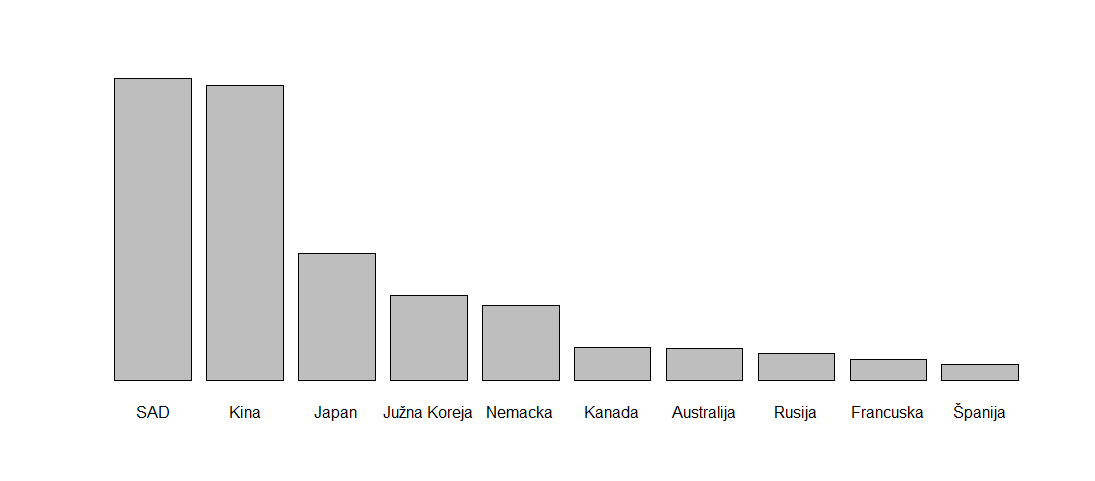
\includegraphics[scale=0.41]{slika.png}
\end{center}
\caption{Broj patenata koje su razvile države u oblasti autonomne vožnje \cite{vehicle_data}} 
\label{fig:histograma}
\end{figure} 

\subsection{Pojava etičkih problema}
\label{subsec:Pojava etičkih problema}
Od pomenutih nivoa automatizacije, prva dva uspešno učestvuju u saobraćaju kao pomoć vozačima, dok iako za treći stepen postoje uslovi, ovakva vozila se smatraju samo korakom napred u razvoju autonomnih vozila iz aspekta nauke, ali nisu od praktičnog značaja iz brojnih \emph{etičkih razloga}. \cite{eticki_problemi_vozila} \\
Naime, takva vožnja zahteva da vozači budu prisutni i da na signal mašine, odnosno vozila, reaguju po potrebi, kako bi rešili neke kritične situacije. Tu se postavljaju pitanja da li je moguce da čovek, koji je na trenutke bio okupiran drugim stvarima i nije pažljivo pratio vožnju sve vreme, može dovoljno brzo da reaguje na zahtev mašine i da li će te reakcije biti ispravne? Poznavajući čovekovu prirodu, nije teško zaključiti da je ovakav koncept prilično nepraktičan i da bi samo povećao broj nesreća umesto da ih minimizuje i učini vožnju udobnom i bezbednom što je cilj.

\subsection{Problem tramvaja}
\label{subsec:Pojava etičkih problema}
Jedan od najpoznatijih problema je problem Tramvaja (eng.~{\em Trolley problem}). To je situacija u kojoj se vozilo kreće šinama i nailazi na šest osoba koje predstavljaju prepreku na putu, ali jedini način da ih ne udari je da skrene na alternativni put na kome se nalazi jedna osoba, koju, takođe, ne može da zaobiđe.  \\
Poznato je da postoje slučajevi u kojima je nemoguće izbeći nezgodu, pa je neophodno utvrditi mehanizam po kome bi mašine donosile odluke i nekada dovodile do eventualnih žrtava. Pitanje koje se na ovome mestu postavlja je - kako postopiti u ovakvoj situaciji, a da postupak bude etički ispravan? Postojanje odgovora na ovo pitanje bi omogućilo opisivanje ponasanja autonomnog vozila koje bi uvek bilo ispravno u kontekstu etike.

\subsection{Etički okviri}
\label{subsec:Etički okviri}
Težina problema kreiranja autonomnih vozila se krije u preslikavanju ispravnih postupaka u matematičke formule koje se nalaze u osnovi odlučivanja automatskih mašina. U literaturi se najčešće porede sledeća tri okvira:
\begin{itemize}
 \item {Deontološka etika - unapred je definisan skup dobrih i loših postupaka}
 \item {Utilitarizam - svaki postupak maksimizuje korist, pa se u različitim              situacijama isti postupak može pokazati nekada ispravan, a nekada ne }
 \item {Etika rizika - procena i minimizacija rizika}
\end{itemize}
Svaki od ova tri okvira, kao i mnogi drugi koji se spominju u literaturi, imaju svoje mane. Do sada \textbf{nije} zabeleženo rešenje neizbežne nesreće koje zadovoljava sve etičke zahteve. \cite{trolley_problem}

\subsubsection{Mane etičkih okvira}
\label{subsubsec:Mane etičkih okvira}
Etika i pravo se ne mogu definisati na jedinstven način - u različitim zemljama se različite stvari smatraju ispravnim, odnosno neispravnim. Mnogo faktora utiče na vozače pri donošenju odluka tokom vožnje, a neke situacije se među vozačima razrešavaju korišćenjem nekih internih načina sporazumevanja poput pokreta ruke, glave i slično, pa je veoma teško napraviti mašinu koja bi donosila odluke poput ljudi u sličnim situacijama. \\
Sledeće važno pitanje je način donošenja odluka u slučajevima poput \textbf{Trolley problema}. Nešto sa čime se ljudi generalno slažu je da bi čovek, bez obzira na bilo kakve karakteristike, trebalo da ima prednost da preživi u odnosu na životinju. Međutim, teško je doneti odluku kada su jedini učesnici ljudi, kao pešaci ili vozači. Same karakteristike pri \emph{izboru žrtve} ne bi smele da imaju uticaj (pol, rasa, starost ili bilo koja druga fizička karakteristika) jer bi u tom slučaju bilo izuzetno zahtevno postaviti granicu - kada nekoga poštedeti, a kada ne, da li više vredi sačuvati živote nekoliko starijih osoba ili jednoj mlađoj i sl. Međutim, ako se detaljnije razmotri takva situacija, mašina bi uvek birala da poštedi veći broj ljudi, iako bi covek na osnovu svog subjektivnog osećaja nekada mogao da postupi \emph{drugacije}. \\
Još jedan aspekt o kome se može diskutovati je pitanje kako se postupa kada je putnik u autonomnoj mašini ugrožen. On nije osoba koja upravlja vozilom, niti osoba koja je napravila ili programirala isto, pa je svakako bitno težiti ponašanju vozila koje pokušava da zaštiti putnika ukoliko je to moguće. Jedan interesantan primer za diskusiju je situacija u kojoj se sa jedne strane vozila nalazi motor, a sa druge kamion - ukoliko vozilo skrene u pravcu motora, veće su šanse da će vozač motora nastradati, međutim ukoliko vozilo skrene u pravcu kamiona, veće su sanse da putnik tog vozila nastrada. \\
Veoma je teško diskutovati na temu etike kada se ljudi nikada neće usaglasiti oko jedinstvenog etičkog okvira, s toga se može izvesti zaključak da potpuna autonomija vozila nikada neće biti prihvaćena od strane svih pojedinaca.

\subsection{Prednosti autonomne vožnje}
\label{subsec:Prednosti autonomne vožnje}
Pored svih kontraverznih pitanja o kojima je bilo reči, autonomna vožnja ima i brojne prednosti: eliminisanje nesreća usled umora ili stresa vozača, prekoračenja brzine, vožnje pod dejstvom psihoaktivnih supstanci. Takođe, ovaj koncept omogućava smanjenje zagađenja zivotne sredine, optimalnu potrošnju i sl.


% Mirjana deo

\section{Veštačka intelijencija u medicini}
\label{sec:upotreba_veštačke_intelijencije_u_medicini}

Veštačka inteligencija pronašla je svoju primenu i u medicini. Primenjuje se u raznim njenim specijalnostima poput dermatologije, radiologije, traumatologije, onkologije, gastroenterologije, dijabetesa, bioinženjeringa, oftamoogije. U nekim od ovih obasti VI se pokazala manje ili više uspešnom, ali za sve njih zajedničko je da je cilj primnene VI bilo olakšanje i poboljšanje procesa  posmatranja, dijagnoze i na kraju samog lečenja bolesti kod obolelih pacijenata. Dok se kao vodeća specijalnost u kojoj se najuspešnije primenjuje VI izdvaja se oftamologija.

Medjutim, uvodjenje VI u medicinu donelo je i veliki broj etiˇckih problema. Naime, prilikom uvodjenja VI kao novog trenda u medicinu nije delovalo da postoje bilo kakvi razlozi za diskusiju po pitanju etike u upotrebi VI u medicini, medjutim kako je vreme prolazilo postalo je oˇcigledno da postoje veliki etiˇcki probemi u tom polju.

Neki od najistaknutijih etičkih problema u primeni VI u medicini opisani su detaljno u narednim poglavljima. Pored problema istaknutih u nastavku postoje i mnogo drugi, ali izdvojeni su samo najinteresantniji.

\subsection{Potrebni podaci}
\label{subsec:poreklo_podataka}

Kako bi se VI uspešno upotrebljavala u medicini potrebno je obezbediti veliku količinu podataka. Ti podaci su potrebni algoritmima VI kako bi trenirali na njima i kako bi se vršila validacija rezultata rada tih algoritma, medjutim tu postoji problem. Naime, potrebni podaci potiču iz različitih resursa poput elektronskih zdravstvenih kartona pacijenata, kliničkih istraživanja i slično. Sa takvim vrstama podataka postoji više različitih etičkih problema, poput vlasništva i javne upotrebe.

Vlasništvo medicinskih podataka predstavlja etički probem jer onaj koji ga poseduje ima moć kontrole, pristupa i obrade tih podataka, a takodje može ostvariti i profit od prava na prodaju tih podataka. Medjutim nije u potpusnoti definisano ko je vlasnik tih podataka. Pored pacijenata čiji su podaci u pitanju pravo na vlasništvo tih podataka mogu tražiti i zdrastvene ustanove u kojima se pacijent leči, lekari, zdravstveni osiguravači pacijenta, korporacije ili pojedinci koji su odgovorni za generisanje, skladištenje i obradu podataka i mnogi drugi.

Ukoliko bi problem vlasništva nad podacima bio rešen, na scenu stupa novi problem, a to je njihova javna upotreba. Da li je potrebno imati dozvole vlasnika podataka da se ti podaci javno koriste, da li je etički prihvatljivo javno korititi te podatke bez pristanka vlasnika?

Korišćenjem tih podataka bez odgovarajućih dozvola mogu nastati razni problemi. Neki od njih su emocionalni stres zbog izlaganja osetljivih zdravstvenih podataka, diskriminacija, lišavanje zdravstvenog osiguranja ili zaposlenja, netraženje zdravstvenih usluga ili uskraćivanje informacija radi zaštite privatnosti i slično.

Ni jedan od ova dva problema nije precizno i uniformno svugde u svetu rešen. Ideja koja se nameće je da bi oni mogli biti rešeni uvodjenjem odgovarajućih zakonskih regulativa koje su u skladu sa etički prihvatljivim ponašanem, i danas se zaista radi na tome u svetu. Medjutim i dalje je sve vezano za tu oblast u povoju i potrebno je dosta rada u tom polju kako bi se ova dva problema, koja se zapravo prepliću uspešno rešila, a samim tim i ubrzao razvoj VI.

\subsection{Veštačka inteligencija i lekari}
\label{subsec:veštačka_inteligencija_i_lekari}

Prilikom pojave svake nove tehnologije dolazi do stavaranja odredjenog stepena zavisnoti od te tehnologije. Tako se pojavila i delimična zavisnot lekara od VI, a ta zavisnost može dovesti do raznih problema. Može se desiti da se lekari previše oslanjaju na rešenja koja im predlaže VI i time postanu nedovoljno oprezni, ili na duže staze može dovesti do gubitka veštine. Takodje, s obzirom na to da su danas veštine lekare potpuno ili delimično zamenjene tehnologijom dolazi do gubitka samopouzdanja i kompetencije lekara.

Pored zavisnoti lekara od VI pojavilo se i suparništvo izmenju njih i VI. Naime, kao što je ranije i navedeno, VI inteligencija se uvela u medicinu sa ciljem da olakša i uapredi rad lekara. Medjutim i u medicini se kao i u raznim drugim obastima stvara strah od preuzimanja posla od ljudi od strane VI.

Pored problema zavisnoti i suparništva, ističu se i problemi poverenja pacijenata, saosećanja i empatije prema pacijentima.

Poverenje koje pacijenti danas imaju u lekare zasniva se na hiljadogodišnjoj praksi. Dok se sa druge strane smatra da za sticanje poverenja u VI od strane pacijenata neće biti potrebno toiko vremena, ali ono danas i dalje ne postoji. Smatra se da je i dalje potrebno dosta rada i truda kako bi se pacijenti uverili u bezbednost primene VI. Glavni razlog zbog kojih pacijenti i dalje nemaju poverenje u VI su pristrasna, netačna, neefikasna, neobjašnjiva i netransparenta rešenja koja u nekim situacijama pruža VI.

Lekari za razliku od mašina i VI imaju saosećanje i osećaj empatije prema pacijentima. Ova činjecice se takodje smatra jednim od glavnih razloga zašto se VI i daje ne prihvata medju pacijentima.

Potrebno je empatične veštine i znanja inkorporirati u programe VI u medicini. Ideja je da se unošenjem hiljada scenarija pacijenta u algoritmime VI oni nauče da imaju empatične reakicije. Tj. ideja je da se razvije "veštačka naklonost" mašina, da mašine nauče da osete i izraze bol i osećanja, tj. da se poboljša "ličnost" mašina. Ovim akcijama mašine bi razvile sposobnost saosećanja sa pacijentima, ali osećaj odgovornosti za štetu nanentu njihovim radnjama.


% Aleksandar deo 


\section{AI korišćen u vojne svrhe}
\label{sec: AI korišćen u vojne svrhe}
Kako se veštačka inteligencija vremenom razvijala, samim tim i njene sposobnosti, logičan korak je bio razmatrati i upotrebu veštačke inteligencije u vojne svrhe. Naravno, kako je vojska obično usko vezana sa događajima od kojih zavise ljudski životi, brzo je dovedena u pitanje i etičnost upotrebe veštačke inteligencije. Naime, prva stvar koja ljudima pada na pamet su neumorni roboti ubice koji su brži i spretniji od ljudi, ali to naravno nije slučaj u stvarnosti.
\newline
\newline
Kada pričamo o veštačkoj inteligenciji u vojne svrhe moramo pričati i komplikacijama koje otežavaju njenu implementaciju. \textbf{Međunarodno humanitano pravo} ili skraćeno \textbf{IHL} (eng. \textit{International Humanitarian Law}) je međunarodno pravo koje se brine o zaštiti civila i njihovih ljutskih prava u ratnim okolnostima. Ono precizno definiše šta jeste a šta nije dozvoljeno vojskama da rade u toku rata. Iako je njegovo postojanje krucijalno za limitiranje štete i nepotrebnog gubitka života, za programere veštačke inteligencije ono predstavlja još jednu prepreku u razvoju bezbednog etičkog softvera.
\newline
\newline
Iako na prvi pogled može da deluje da veštačka inteligencija unosi samo komplikacije i negativne posledice, pretežno za manje razvijene države koje ne mogu da je priušte, ispostavlja se da to ipak nije uvek slučaj. Kao i kod većine drugih etičkih pitanja problem ima svoje \emph{negativne} i \emph{pozitivne} strane.
\subsection{Negativne strane vojnog AI}
\label{subsec: Negativne strane vojnog AI}
Iako su neumorni roboti ubice element naučne fantastike, to ne znači da vojna veštačka inteligencija nema svoje loše strane. Koncept veštačke inteligencije je relativno nov i veoma kompleksan, što ga čini sklonim greškama, a minimalna greška može imati katastrofalne posledice ne samo po vojnike koji sa tim AI rade, već i po nedužne civile dovoljno nesretne da budu umešani. Glavni problemi ovakvog oblika veštačke inteligencije su problemi \emph{odgovornosti} i \emph{pretprilagođenosti}. 

\subsubsection{Problem odgovornosti}
\label{subsubsec: Problem odgovornosti}
Kao što samo ime kaže ovaj problem obuhvata ideju da nije precizno definisano ko snosi posledice onoga što veštačka inteligencija ``samostalno`` uradi.  Ukoliko postoji potpuno autonomni sistem koji krši pravila vođenja borbe (eng. \emph{rules of engagement}) ili međunarodnog humanitarnog prava pitanje je ko je kriv. Ukoliko sistem ispravno radi, da li je kriv samo general koji je izdao nehumana naređenja ili je kriv i programer što nema provere zadovoljenosti IHL? Ako pak sistem radi neispravno da li je kriv programer koji je napravio grešku ili general koji je dozvolio upotrebu nebezbednog sistema? Moguće posledice ovakvih problema nisu zanemarljive zato je veoma važno imati precizno definisanog krivca.
\newline
\newline
Iako problem nije u potpunosti rešiv u slučaju neispravnog softvera, programeri deo ovog problema ublažuju uvođenjem nekog vida ljudske medijacije. Naime sistemi se prave tako da uvek postoji odgovorna osoba koja će u krucijalnim momentima doneti odgovarajuću odluku. Tako npr. automatizovani mitraljezi koji čuvaju određenu teritoriju često automatski daju upozorenje ukoliko neko kroči na tu teritoriju, a pucaju samo ukoliko dobiju odobrenje od zadužene osobe.

\subsubsection{Problem pretprilagođenosti}
\label{subsubsec: Problem pretprilagođenosti}
Problem pretprilagođenosti podrazumeva nepredvidivo ponašanje algoritama koji uče na osnovu nekih ulaznih podataka. Problemi ove vrste često dovode do sistema koji često previđa neke krupne detalje koji bi bili očigledni čoveku. Primeri problema koji mogu nastati su pogrešno razlikovanje civila i vojnika (npr. po rasi umesto po uniformi), nerazlikovanje vojnih baza i civilnih naselja, previđanje očiglednih prepreka (npr. kod automatske navigacije) i slično.
\newline
\newline
Za razliku od ljudi, koji su fleksibilni i umeju da se adaptiraju, ovi sistemi sadrže samo nekoliko scenarija na koje znaju da reaguju. Način rešavanja ovog problema je isti kao i kod svih drugih sistema koji uče, a to je adekvatan odabir ulaznih podataka i algoritma za učenje, kao i temeljno testiranje svih potencijalno problematičnih situacija.

\subsection{Pozitivne strane vojnog AI}
\label{subsec: Pozitivne strane vojnog AI}
Iako kvalitetna veštačka inteligencija može da doprinosi lakom osvajanju bitaka, to nije nužno pozitivna strana za manje razvijene države koje bi joj se potencijalno suprotstavljale. Ključan deo pozitivne strane pretstavlja koncept \textbf{etičkog oružija}. Etičko oružije je oružije koje je pametno programirano sa svim pravilima i zakonima ratovanja kao što su su pravila vođenja borbe i IHL. Ovakvi sistemi su zasnovani na tehnologijama maksimalno i minimalno pravičnog AI (eng. \textit{maximally just AI} i \textit{minimally just AI}), odnosno \textbf{MaxAI} i \textbf{MinAI}.

\subsubsection{MaxAI i MinAI}
\label{subsubsec: MaxAI i MinAI}
Za razliku od proizvoljnih sistema MaxAI i MinAI ne ispunjavaju ``slepo`` naređenja koja su im zadata. Ovi sistemi su programirani da uzimaju u obzir različite okolnosti i zakone i adekvatno sa time ``modifikuju`` naređenja.
\newline
\newline
U slučaju MaxAI ukoliko se primeti da naređenja ne zadovoljavaju zadate zakone, algoritam se trudi da što preciznije prati naređenja uz minimalne izmene. Izmene mogu obuhvatati smanjenje primenjene sile do minimalno neophodne ili odbijanje napadanja zaštićenih objekata poput objekata crvenog krsta, bolnica i slično. MaxAI postoji pretežno u teoriji baš zbog toga što je izuzetno teško uzeti u obzir sve apstraktne parametre i posledice naređenja i ublažiti ih na minimalno neophodne.
\newline
\newline
MinAI obično podrazumeva mnogo jednostavniji sistem sa limitiranim opcijama i ishodima, što ga čini mogućim za implemenitranje za razliku od MaxAI. Naime MinAI obično podrazumeva zadavanje naređenja i ukoliko naređenje krši neke zadate zakone ono se jednostavno ne izvršava. U nekim implementacijama moguće je zadavanje i sekundarnog naređenja (eng. \textit{failsafe}) na čiju se proveru i izvršavanje prelazi ukoliko prvo naređenje nije izvršivo.

\section{Zaključak}
\label{sec: Zaključak}
Etički problemi u veštačkoj inteligenciji su brojni, opširni i veoma teški za rešavanje iz više razloga. Za početak oblasti od kojih su sačinjeni ovi problemi, etika i veštačka inteligencija, su same po sebi veoma kompleksne. Sa jedne strane, imamo etiku, nauku zasnovanu na pitanju morala koji se po svojoj definiciji razlikuje od pojedinca do pojedinca i nema precizno definisane ispravne i pogrešne odgovore na neka pitanja. Sa druge strane, imamo veštačku inteligenciju, relativno svestranu i kompleksnu granu programiranja koja obuhvata i pokušava da reši mnoštvo različitih, ponekad previše opštih, problema. Sa ovim na umu, postavlja se pitanje kako naučiti mašinu da etički rešava problem ako mi sami ne možemo da se usaglasimo po pitanju etike, a istovemeno ne možemo da sagledamo sve strane tog kompleksnog problema?
\newline
Problemi etike u veštačke inteligenciji su brojni i do sada spomenuti su samo neki od njih. Etički problemi su prisutni u praktično svakoj situaciji, ukoliko je sagledamo iz određenog ugla, neki od kojih su očigledniji od drugih. Pored obrađenih problema u oblastima društvenih mreža, autonomnih vozila, medicine i vojske postoje i brojne druge oblasti sa svojim problemima kao što su umetnost, radna snaga, obrada slike i zvuka, ekonomija i mnogi drugi za koje je potrebna detaljnija diskusija.

\newpage

\addcontentsline{toc}{section}{Literatura}
\appendix
\bibliography{seminarski} 
\bibliographystyle{plain}

\appendix



\end{document}
